\documentclass[12pt]{article}

%%======== PACKAGES & PAGE SETUP ========
\usepackage[utf8]{inputenc}
\usepackage[T1]{fontenc}
\usepackage{newtxtext}
\usepackage{amsmath,amssymb,amsfonts,amsthm}
\usepackage{mathtools}
\usepackage{bm}
\usepackage{enumitem}
\usepackage[a4paper, hmargin=2.5cm, vmargin=3cm]{geometry}
\usepackage{setspace}
  \setstretch{1.35}
\usepackage{graphicx,booktabs,float}
\usepackage{xcolor}
  \definecolor{buRed}{HTML}{CC0000}
\usepackage{tikz}
  \usetikzlibrary{calc}
\usepackage{hyperref}
  \hypersetup{colorlinks=true, linkcolor=blue, urlcolor=blue, citecolor=blue, pdfborder={0 0 0}}
\usepackage{listings}
\lstdefinestyle{pseudo}{basicstyle=\ttfamily\footnotesize, columns=fullflexible,
  keepspaces=true, breaklines=true, frame=single, framesep=5pt,
  rulecolor=\color{gray!50}, showstringspaces=false}
\lstdefinestyle{code}{language=Python, basicstyle=\ttfamily\scriptsize,
  keywordstyle=\color{blue!70!black}, commentstyle=\color{gray}, stringstyle=\color{buRed!80!black},
  showstringspaces=false, breaklines=true, numbers=left, numberstyle=\tiny\color{gray},
  frame=single, rulecolor=\color{gray!50}}
\usepackage{fancyhdr}
  \pagestyle{fancy}
  \fancyhf{}
  \fancyfoot[C]{\thepage}
  \renewcommand{\headrulewidth}{0pt}

%%======== HOMEWORK MACROS ========
\newcommand{\hwNumber}{\#13}
\newcommand{\hw}{Homework}
\newcommand{\E}{\mathbb{E}}
\newcommand{\PP}{\mathbb{P}}
\newcommand{\VaR}{\mathrm{VaR}}
\newcommand{\1}{\mathbf{1}}
\theoremstyle{remark}
\newtheorem*{remark}{Remark}

%%======== BU LOGO ========
\newcommand{\buLogo}[2][]{%
  \begin{tikzpicture}[#1]
    \pgfmathsetlengthmacro{\BUwidth}{#2}
    \pgfmathsetlengthmacro{\BUheight}{#2 * 1.5 / 5}
    \fill[buRed] (0,0) rectangle (\BUwidth,\BUheight);
    \draw[white, line width=1.5pt] (0,0) rectangle (\BUwidth,\BUheight);
    \draw[white, line width=0.8pt]
      ($(0,0)+(2pt,2pt)$) rectangle ($(\BUwidth,\BUheight)+(-2pt,-2pt)$);
    \node[text=white, anchor=center, font=\fontsize{30pt}{44pt}\selectfont]
      at (0.5*\BUwidth, 0.70*\BUheight) {BOSTON};
    \node[text=white, anchor=center, font=\normalfont\fontsize{20pt}{28pt}\selectfont,
      text width=\BUwidth, align=center]
      at (0.5*\BUwidth, 0.30*\BUheight) {UNIVERSITY};
  \end{tikzpicture}%
}

\newcommand{\N}{503}
\newcommand{\Nprices}{504}
\newcommand{\EmpK}{488}
\newcommand{\EmpRank}{16}
\newcommand{\Xbar}{0.1341}
\newcommand{\Sn}{1.2961}
\newcommand{\Zq}{-1.8808}
\newcommand{\Zalpha}{1.8808}
\newcommand{\QLo}{431.24}
\newcommand{\QHi}{578.64}
\newcommand{\SigLo}{1.2073}
\newcommand{\SigHi}{1.3984}
\newcommand{\VarEmp}{24,984.39}
\newcommand{\VarPt}{22,773.55}
\newcommand{\VarLo}{21,138.53}
\newcommand{\VarHi}{24,651.99}
\newcommand{\WidthA}{3,513}
\newcommand{\YBar}{22,808.77}
\newcommand{\YSE}{2.67}
\newcommand{\YMed}{22,787.89}
\newcommand{\BA}{20,698.11}
\newcommand{\BB}{25,091.16}
\newcommand{\WidthB}{4,393}
\newcommand{\WidthRatio}{1.25}
\newcommand{\EmpOver}{332}
\newcommand{\CoverA}{98.02}
\newcommand{\CoverB}{97.75}
\newcommand{\SimALo}{21,145}
\newcommand{\SimAHi}{24,654}
\newcommand{\Skew}{0.21}
\newcommand{\ExKurt}{2.88}
\newcommand{\JBp}{3.6\times10^{-39}}
\newcommand{\NExceed}{20}
\newcommand{\NExpect}{15.1}
\newcommand{\SigBias}{0.150}
\newcommand{\YMinusPt}{35}
\newcommand{\SeedMeans}{22,815, 22,807, 22,805}
\newcommand{\AdjEmp}{24,984}
\newcommand{\AdjPt}{22,650}
\newcommand{\AdjLo}{21,019}
\newcommand{\AdjHi}{24,524}
\newcommand{\AdjY}{22,685}
\newcommand{\AdjA}{20,579}
\newcommand{\AdjB}{24,962}
\newcommand{\Realized}{15,352}
\newcommand{\NextRet}{1.54}
\newcommand{\M}{125,000}
\newcommand{\Seed}{731}


%%======== DOCUMENT ========
\begin{document}

\begin{titlepage}
\begin{center}
  \vspace*{2cm}
  \buLogo{7cm}

  \vspace{1em}
  \textbf{Questrom School of Business\\}
  \vfill
  \textbf{MF731: Corporate Risk Management \\}
  \textbf{Qingshuo Song \\}
  {\hw\ \hwNumber: How Sure Are We About VaR? Confidence Intervals for Apple \\}
  \vfill
  \textbf{Nabizhan Bobokhanov \\}
  (Student ID: U19132437) \\
  \vfill
  \fbox{\parbox{0.8\textwidth}{\centering\small \textbf{Code:} \url{https://github.com/nabizhka/ci-hw}\\ (the full source is also listed in the Appendix)}}
\end{center}
\end{titlepage}

\section*{Setup and data}
$V_t=\$1{,}000{,}000$ is held in Apple (AAPL) at the close of 10/31/2018, and the loss is over one day,
10/31/2018 to 11/1/2018:
\[
L_{t+\Delta}=-V_t\bigl(e^{X_{t+\Delta}}-1\bigr),\qquad X_{t+\Delta}\mid\mathcal F_t\sim N(\mu,\sigma^2).
\]
Since $L$ is decreasing in $X$, $\VaR_\alpha(L)=-V_t\bigl(e^{q_{1-\alpha}(X)}-1\bigr)$ with
$q_{1-\alpha}(X)=\mu+\sigma\Phi^{-1}(1-\alpha)$, which is formula (1):
\[
\VaR_\alpha=V_t\bigl(1-e^{\mu+\sigma\Phi^{-1}(1-\alpha)}\bigr),\qquad \Phi^{-1}(1-\alpha)=\Zq\ \text{ at }\alpha=.97 .
\]
Because $\Phi^{-1}(1-\alpha)<0$, VaR is \emph{increasing in $\sigma$} and decreasing in $\mu$. Every
interval below comes from this monotonicity.

\textbf{Data.} Yahoo Finance daily closes (\texttt{Close}, split-adjusted, not dividend-adjusted),
11/1/2016 to 10/31/2018, frozen in \texttt{data/}. That is \Nprices\ closes and $n=\N$ log returns
$X_i=\log(P_i/P_{i-1})$. The standard estimators are
\[
\bar X_n=\frac1n\sum_{i=1}^nX_i=\Xbar\%,\qquad
S_n=\Bigl(\frac1{n-1}\sum_{i=1}^n(X_i-\bar X_n)^2\Bigr)^{1/2}=\Sn\%\ \text{(daily)}.
\]
Parameters: $\alpha=.97$, $\beta=.02$ (so 98\% intervals), $M=\M$, seed \Seed.

%-------------------------------------------------------------------------------
\section*{(a) $\mu$ known ($=\bar X_n$), $\sigma$ unknown}

\textbf{Empirical estimate.} With the course definition $\VaR_\alpha=\inf\{\ell:F_n(\ell)\ge\alpha\}$,
the estimate is the order statistic $\ell_{(\lceil n\alpha\rceil)}$ of the $n$ historical losses
$\ell_i=-V_t(e^{X_i}-1)$. Here $\lceil\N\times.97\rceil=\EmpK$, the \EmpRank th largest loss:
\[
\widehat{\VaR}^{\,\mathrm{emp}}_{.97}=\$\VarEmp .
\]

\textbf{Formula (1) with the sample moments.}
\[
\widehat{\VaR}_{.97}=V_t\bigl(1-e^{\bar X_n+S_n\Phi^{-1}(.03)}\bigr)=\$\VarPt .
\]

\textbf{Confidence interval.} For i.i.d.\ $N(\mu,\sigma^2)$ data, $(n-1)S_n^2/\sigma^2\sim\chi^2_{n-1}$
(lecture: $\sum_i((X_i-\mu)/\sigma)^2=(n-1)S_n^2/\sigma^2+\bigl((\bar X_n-\mu)/(\sigma/\sqrt n)\bigr)^2$,
a $\chi^2_n$ split into independent $\chi^2_{n-1}$ and $\chi^2_1$ pieces). With $q_p$ the $p$-quantile of
$\chi^2_{n-1}$,
\[
\PP\Bigl[q_{\beta/2}\le\tfrac{(n-1)S_n^2}{\sigma^2}\le q_{1-\beta/2}\Bigr]=1-\beta
\iff
\PP\bigl[\underline\sigma\le\sigma\le\overline\sigma\bigr]=1-\beta,
\]
where
\[
\underline\sigma=\sqrt{\tfrac{n-1}{q_{1-\beta/2}}}\,S_n,\ \
\overline\sigma=\sqrt{\tfrac{n-1}{q_{\beta/2}}}\,S_n .
\]
With $n-1=502$: $q_{.01}=\QLo$, $q_{.99}=\QHi$, so $\underline\sigma=\SigLo\%$ and
$\overline\sigma=\SigHi\%$. Note the order flips: the \emph{upper} $\chi^2$ quantile gives the
\emph{lower} $\sigma$. Since VaR is increasing in $\sigma$, the event $\{\underline\sigma\le\sigma\le\overline\sigma\}$
is the same event as $\{\VaR(\underline\sigma)\le\VaR_\alpha\le\VaR(\overline\sigma)\}$, so
\[
98\%\ \text{CI}:\quad
\Bigl(V_t\bigl(1-e^{\bar X_n+\underline\sigma\Phi^{-1}(.03)}\bigr),\ V_t\bigl(1-e^{\bar X_n+\overline\sigma\Phi^{-1}(.03)}\bigr)\Bigr)
=(\$\VarLo,\ \$\VarHi).
\]

%-------------------------------------------------------------------------------
\section*{(b) $\mu$ and $\sigma$ both unknown}

The method from class (Model Risk deck, slide 30). For $m=1,\dots,M$:
\begin{enumerate}[leftmargin=*,itemsep=0pt]
\item draw $\sigma^m$ from $(n-1)S_n^2/(\sigma^m)^2\sim\chi^2_{n-1}$, i.e.\ $\sigma^m=S_n\sqrt{(n-1)/W_m}$ with $W_m\sim\chi^2_{n-1}$;
\item draw $\mu^m\sim N\bigl(\bar X_n,(\sigma^m)^2/n\bigr)$, since $(\bar X_n-\mu)/(\sigma/\sqrt n)\sim N(0,1)$;
\item set $Y_m=\VaR^m_\alpha=V_t\bigl(1-e^{\mu^m+\sigma^m\Phi^{-1}(1-\alpha)}\bigr)$.
\end{enumerate}
\begin{lstlisting}[style=pseudo]
INPUT closes P_0..P_n, V = 1e6, alpha = .97, beta = .02, M = 125000, seed 731
X_i = log(P_i / P_(i-1));  xbar = mean(X);  S = sd(X, ddof = 1);  z = Ninv(1 - alpha)
W   = chi2(n - 1).sample(M)
sig = S * sqrt((n - 1) / W)
mu  = Normal(xbar, sig / sqrt(n)).sample()          # one draw per sig
Y   = V * (1 - exp(mu + sig * z))
OUTPUT mean(Y),  A = quantile(Y, beta/2),  B = quantile(Y, 1 - beta/2)
\end{lstlisting}
Results:
\[
\bar Y_M=\$\YBar\ \ (\text{MC standard error } \$\YSE),\qquad (A,B)=(\$\BA,\ \$\BB).
\]

%-------------------------------------------------------------------------------
\section*{Comparison}

\begin{figure}[H]\centering
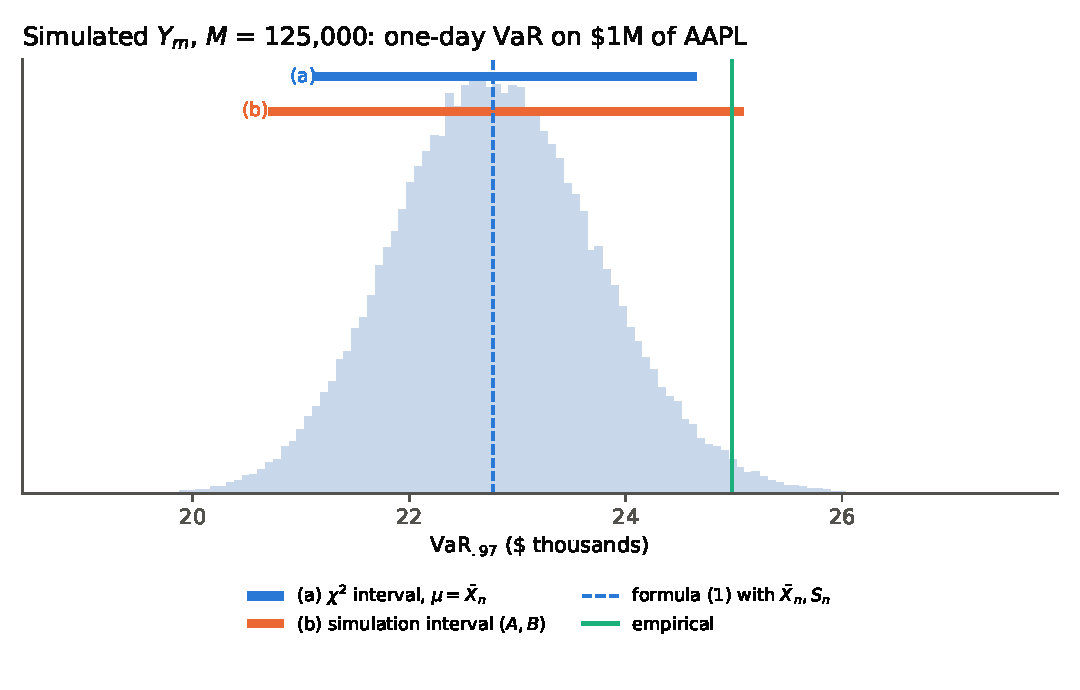
\includegraphics[width=\linewidth]{figures/var_ci.pdf}
\caption{The $M$ simulated values $Y_m$ with both 98\% intervals, the point estimate from (1) and
the empirical estimate.}
\end{figure}

\begin{table}[H]\centering\small
\begin{tabular}{lrrrr}\toprule
Method & estimate (\$) & low (\$) & high (\$) & width (\$)\\\midrule
(a) empirical & \VarEmp & & & \\
(a) formula (1), $\chi^2$ interval for $\sigma$ & \VarPt & \VarLo & \VarHi & \WidthA\\
(b) simulation, $\mu$ and $\sigma$ unknown & \YBar & \BA & \BB & \WidthB\\\bottomrule
\end{tabular}
\caption{One-day $\VaR_{.97}$ on \$1M of AAPL, 98\% intervals.}
\end{table}

\begin{center}
\fbox{\parbox{0.9\textwidth}{
\textbf{(a)} empirical \$\VarEmp; formula \$\VarPt, 98\% CI (\$\VarLo, \$\VarHi).\\[2pt]
\textbf{(b)} $\bar Y_M=$ \$\YBar, 98\% interval (\$\BA, \$\BB).}}
\end{center}

\textbf{The point estimates agree; the intervals do not.} $\bar Y_M$ is only \$\YMinusPt\ above the
plug-in value. It comes from the sampling scheme, and it is larger than the MC error: $\E[\sigma^m]/S_n=\sqrt{\tfrac{n-1}2}\,\Gamma(\tfrac{n-2}2)/\Gamma(\tfrac{n-1}2)$,
which is $\SigBias\%$ above one at $n=\N$, and $\partial\VaR/\partial\sigma\approx V_t|\Phi^{-1}(.03)|$
turns that into about \$36. The randomness in $\mu^m$ adds almost nothing to the mean because
$\mu$ enters through $e^{\mu}$ and $\mathrm{sd}(\mu^m)=\sigma/\sqrt n\approx0.06\%$.

The interval in (b) is \WidthRatio\ times as wide as in (a), \$\WidthB\ against \$\WidthA. In (a)
the only uncertainty is in $\sigma$. In (b) the mean is also unknown, and its standard error
$\sigma/\sqrt n=0.058\%$ is not small next to the $\sigma$ effect: shifting $\mu$ by one standard error
moves VaR by about $V_te^{\mu+\sigma\Phi^{-1}(.03)}\times0.058\%\approx\$565$, a sixth of the width in (a). Both effects are
$O(1/\sqrt n)$, so neither can be ignored with two years of data.

\textbf{The empirical estimate sits outside the interval in (a)} by \$\EmpOver, and just inside
(b). The intervals measure only parameter uncertainty \emph{inside} the normal model. They say
nothing about whether the normal model is right, and for AAPL it is not: sample skewness \Skew,
excess kurtosis \ExKurt, Jarque--Bera $p=\JBp$. Over the sample, \NExceed\ daily losses exceeded
the formula's VaR against $n(1-\alpha)=\NExpect$ expected. At $97\%$ the fat tail is already
pushing the empirical quantile above the normal one. So the honest reading is: given normality,
we know VaR to within about $\pm\$2{,}000$; the gap to the empirical number is model risk of a
different kind, mis-specification, which no $\chi^2$ interval can see.

%-------------------------------------------------------------------------------
\section*{Checks}
\begin{itemize}[leftmargin=*]
\item \textbf{(a) by simulation.} Simulating $\sigma^m$ alone with $\mu=\bar X_n$ fixed gives a 1\%--99\%
range of (\$\SimALo, \$\SimAHi), matching the closed-form interval. So (b) differs from (a) only by
the $\mu$ step.
\item \textbf{Coverage.} I generated 20{,}000 samples of $n=\N$ i.i.d.\ normal returns with known true
parameters (set to $\bar X_n$, $S_n$) and rebuilt interval (a) on each: it covered the true VaR
\CoverA\% of the time against a nominal 98\%. Interval (b), rebuilt on 2{,}000 samples with
$M=20{,}000$ each, covered \CoverB\% (standard error about 0.3\%).
\item \textbf{Seeds.} Three other seeds give $\bar Y_M$ of \$\SeedMeans; the MC standard error is \$\YSE.
\item \textbf{Adjusted closes.} With dividend-adjusted closes: empirical \$\AdjEmp; formula \$\AdjPt,
CI (\$\AdjLo, \$\AdjHi); simulation \$\AdjY, (\$\AdjA, \$\AdjB). The dividend days raise
$\bar X_n$ slightly and lower VaR by about \$120. The empirical value then falls outside both
intervals. Conclusions unchanged.
\item \textbf{What happened.} AAPL rose \NextRet\% on 11/1/2018, a gain of \$\Realized. Not a test of
anything with one day, just a sanity check on dates.
\end{itemize}

\textbf{Readings of the sheet.} ``Apple index'' is read as Apple stock. ``The empirical distribution of
log returns'' is used through the full loss $-V_t(e^{X}-1)$, the same operator as (1), so the two
estimates in (a) differ only by the distribution. The window ends at the 10/31/2018 close, the
start of the loss period.

\begin{center}
\fbox{\parbox{0.92\textwidth}{\textbf{Carry.}
(1) The pivot is $(n-1)S_n^2/\sigma^2\sim\chi^2_{n-1}$. Invert it for $\sigma$, then push the endpoints
through VaR, which is monotone in $\sigma$. The upper $\chi^2$ quantile gives the lower $\sigma$.
(2) It assumes i.i.d.\ normal data. Fat tails break it, and the interval is then too narrow: it
cannot contain the empirical VaR, as here.
(3) With $\mu$ unknown too, simulate: $\sigma^m$ from $\chi^2_{n-1}$, then $\mu^m\mid\sigma^m\sim N(\bar X_n,(\sigma^m)^2/n)$.
(4) Exam phrasing: ``which bound uses $q_{\beta/2}$?'' or ``why is (b) wider?''. Answer with the
monotonicity of VaR in $\sigma$ and $\mu$.}}
\end{center}

\appendix
\section{Python source code}
Data download, \texttt{src/get\_data.py}:
\lstinputlisting[style=code]{src/get_data.py}
Estimates and checks, \texttt{src/ci.py}:
\lstinputlisting[style=code]{src/ci.py}
Report values and figure, \texttt{src/main.py}:
\lstinputlisting[style=code]{src/main.py}

\end{document}
